\begin{center}
  \Large
  \textbf{BIOGRAFI PENULIS}
\end{center}

\addcontentsline{toc}{chapter}{BIOGRAFI PENULIS}

\vspace{2ex}

\begin{wrapfigure}{L}{0.3\textwidth}
  \centering
  \vspace{-3ex}
  % Ubah file gambar berikut dengan file foto dari mahasiswa
  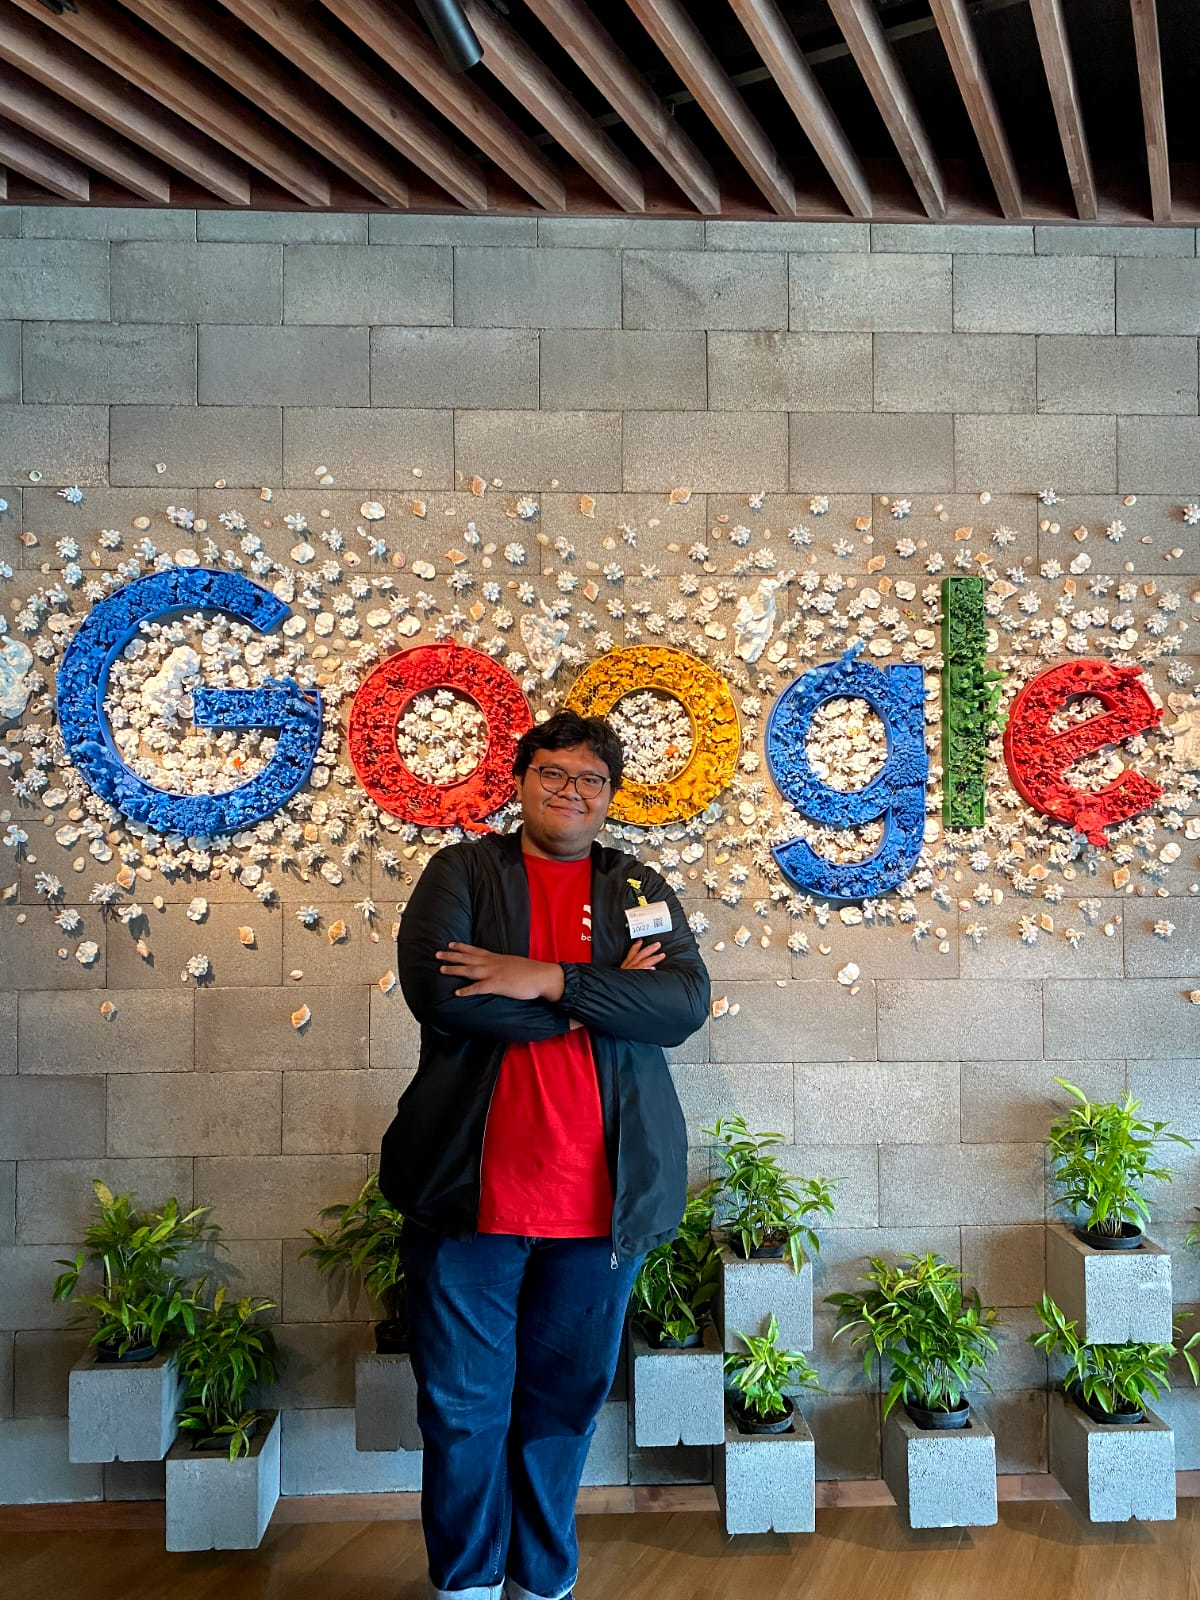
\includegraphics[width=0.3\textwidth]{gambar/foto_biografi.jpg}
  \vspace{-4ex}
\end{wrapfigure}

% Ubah kalimat berikut dengan biografi dari mahasiswa
\name{}, lahir di kota Tulungagung pada 24 Maret 2002, adalah seorang mahasiswa yang memiliki kecintaan mendalam terhadap teknologi dan inovasi. Saat ini, Arya menempuh pendidikan di Institut Teknologi Sepuluh Nopember, di jurusan Teknik Komputer, yang dikenal dengan keunggulan akademis dan kontribusinya dalam teknologi informasi.

Di luar kelas, Arya mengejar berbagai hobi yang memperkaya wawasan dan keterampilannya, seperti mendengarkan musik, membaca buku, dan yang terutama adalah mengeksplorasi kemajuan terbaru dalam teknologi. Kecintaannya terhadap musik dan buku membuka perspektif baru dan menambah kedalaman pemahamannya tentang dunia.

Arya telah terlibat dalam sejumlah proyek yang menunjukkan keahliannya dalam pengembangan backend menggunakan Node.js, serta pengalaman dalam DevOps dan cloud computing dengan menggunakan platform Google Cloud. Keahliannya tidak terhenti di situ; ia juga mengembangkan kemampuan dalam bidang machine learning dan robotic operating system, yang menunjukkan keberanian dan kecakapan teknisnya dalam menghadapi tantangan baru.

Lebih lanjut, Arya juga mendalami pengembangan frontend menggunakan React JS, mengintegrasikan desain yang responsif dengan pengalaman pengguna yang intuitif. Terbaru, ia mulai mengeksplorasi ranah blockchain dan smart contract dengan menggunakan Solidity, menandai langkah selanjutnya dalam perjalanan teknologinya.

Dengan basis pengetahuan yang luas dan terus berkembang, Arya berambisi untuk menjadi inovator dan pemimpin di dunia teknologi, menggunakan setiap proyek dan kesempatan pembelajaran sebagai batu loncatan menuju keberhasilan yang lebih besar.
